\documentclass[11pt, titlepage]{article}
\usepackage{ngerman}   	% use "amsart" instead of "article" for AMSLaTeX format
\usepackage{geometry}    
\usepackage[latin1]{inputenc} 
\usepackage{amsmath}
\usepackage{wasysym}
\usepackage{amstext}
\usepackage{cmbright}
\usepackage[T1]{fontenc}
\newcommand{\changefont}[3]{
\fontfamily{#1} \fontseries{#2} \fontshape{#3} \selectfont}

           		% See geometry.pdf to learn the layout options. There are lots.
\geometry{letterpaper}                   		% ... or a4paper or a5paper or ... 
%\geometry{landscape}                		% Activate for for rotated page geometry
%\usepackage[parfill]{parskip}    		% Activate to begin paragraphs with an empty line rather than an indent
\usepackage{graphicx}				% Use pdf, png, jpg, or eps§ with pdflatex; use eps in DVI mode
\usepackage{amssymb}								% TeX will automatically convert eps --> pdf in pdflatex	
								
									
\title{\textbf {Unreal Engine 4.7}\\
\ \\
Eine Anleitung f"ur Project Unik\\}
\author{Elham Nizam}

							
\begin{document}

\maketitle
%\section{}
%\subsection{}
\tableofcontents \newpage

\changefont{ptm}{m}{n}

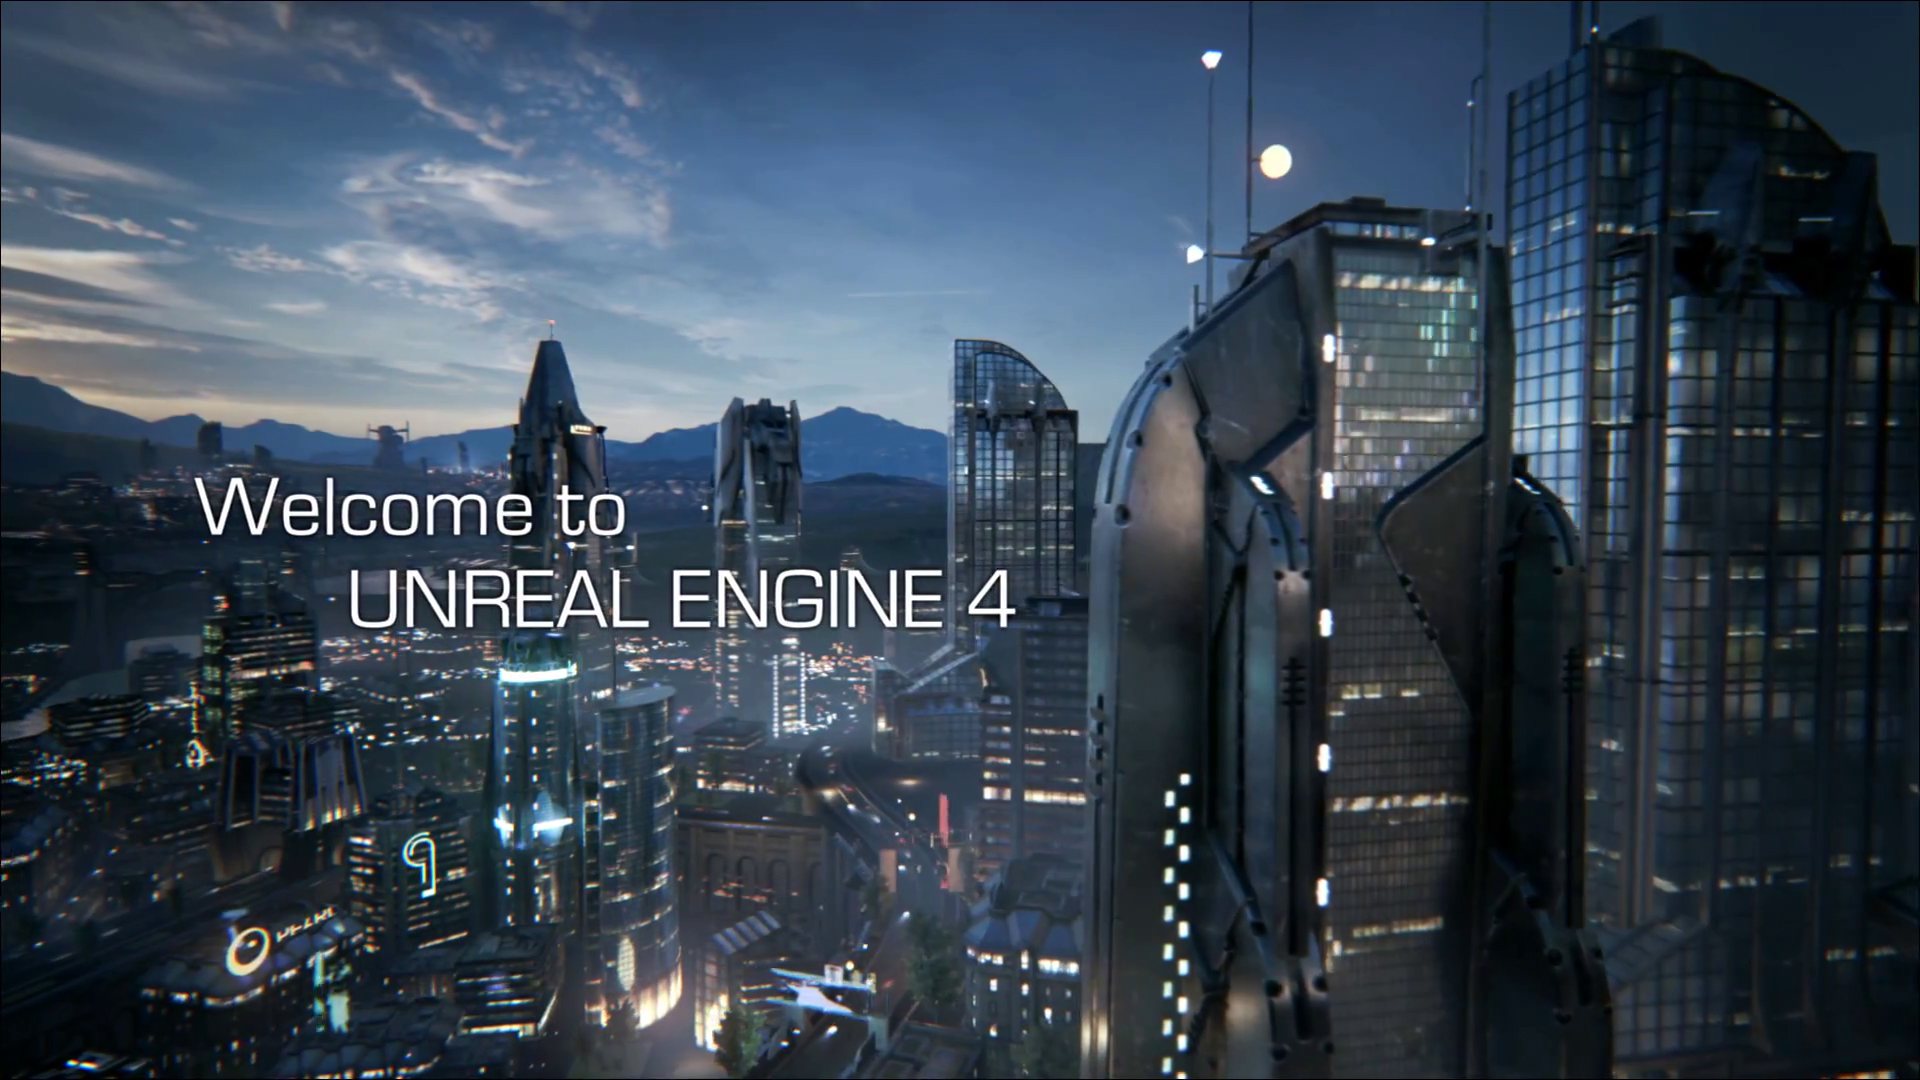
\includegraphics[height=7cm, width=14cm]{1395248778-u4}

\section{Vorwort}

\noindent Hallo alle zusammen, \newline
\noindent anl"asslich des Projekt Unik und dem Ziel ein marktf"ahiges Videospiel zu entwickeln, hab ich mich entschlossen, mich umfassend mit der Engine zu befassen und euch diesen Guide zu schreiben. Die meisten Infos und Anleitungen sind direkt den Video-Tutorials der Unreal-Homepage entnommen, einiges auch durch Eigenrecherche erg"anzt. In den letzten Tagen kam auch wiederholt die Frage auf, ob Unreal so n"utzlich ist, wie anfangs gedacht, oder vielleicht doch zu schwierig f"ur ein junges, unerfahrenes Team. Ich muss zugeben, die Frage besch"aftigte mich eine ganze Weile. Generell, und das hab ich schon oft verlauten lassen, bin ich ein starkes Bef"urworter f"ur Ambition. Es gibt jedoch eine feine Grenze zwischen Ambition und Gr"o"senwahn, deshalb hab ich w"ahrend der Gamescom die Gelegenheit ergriffen und mit anderen (teils ebenfalls) jungen Indie-Entwicklern gesprochen und auch oft die Unreal-Frage angesprochen. \newline
\noindent Am pr"agendsten war das Gespr"ach mit dem Chief Developer von We happy few, einem neuen Indie-Titel, durch Kickstarter finanziert, und nun auf ID@Xbox zu sehen. Compulsion Games, ein Team aus 14 Leuten, hat in We Happy Few ein dystopisches, retrofuturistisches London der 60er geschaffen. Das Gameplay und die Story laufen in einer gro"sen, dynamischen Open-World ab und werden durch eine brilliante KI erg"anzt. Ich will jetzt keine Werbung f"ur das Spiel machen, allerdings war ich erstaunt, was dieses Team hingekriegt hat. Mir ist bewusst, dass es einen Unterschied zwischen Unik und einem professionellen Indie-Entwickler-Team gibt, dennoch bin ich der Meinung, dass wir mehr als in der Lage sind, ein (halb-)lineares Horrospiel zu kreieren, zumal unsere Herausforderungen in anderen Bereichen liegen werden. Auch die drei anwesenden Entwickler von Compulsion Games rieten mir weiterhin am Ball zu bleiben, und keineswegs wegen m"oglicher Schwierigkeiten mit der Engine vom Kurs abzuweichen. \newline
\noindent Was ich letzendlich damit sagen mag, wir weichen nicht vom Kurs ab und behalten Unreal weiterhin als Engine. Die Forumbeitr"age hab ich nat"urlich zur Kenntnis genommen, und ich stimme definitiv auch den Problemen zu. Nach umfassender Recherche bin ich aber auch zu dem Schluss gekommen, dass Unreal diese Problemzone durch seine anderen, weitaus gr"o"seren Vorteile wieder wett macht.


\section{Grundlegendes}

\noindent Dieses Kapitel befasst sich mit der grundlegenden Steuerung innerhalb des Unreal-Interfaces. Alle Anleitungen sind bez"uglich des Standardinterfaces geschrieben und sollen die allgemeine Steuerung innerhalb der Engine n"aher bringen. Manches mag einem banal vorkommen, dennoch ist eine intuitive Benutzung aller gebotenen Features ausschlaggebend f"ur ein funktionierendes Spiel, daher bitte ich alle darum, aufmerksam die folgenden Seiten zu lesen.

\subsection{"Uberblick der UI}

\noindent Beim Starten der Engine "offnet sich zun"achst der Unreal Project Browser, der uns erlaubt ein neues Projekt zu starten oder ein bereits begonnenes fortzuf"uhren. \newline
\newline
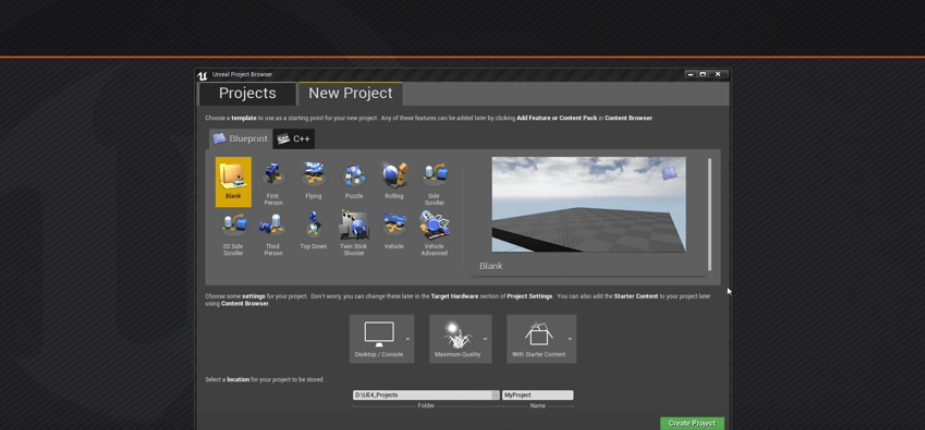
\includegraphics[height=7cm, width=15cm]{Capture}
\newline
\noindent Unreal bietet uns hier eine Reihe von vorgefertigten Templates an, wir benutzen jedoch ein blankes Projekt (Starter Content enabled). \newline
\newline
\noindent Linksklick Blank $\rightarrow$ Starter Content enabled $\rightarrow$ Projekt benennen $\rightarrow$ Create Project \newline
\newpage
\noindent Das Interface sollte wie folgt aussehen: \newline
\newline
\includegraphics[height=12cm, width=16cm]{Capture2}
\newline
\noindent 1 Viewport: Level Editing Fenster, erlaubt den Blick in die 3D Welt \newline
\noindent 2 Menu Bar: Enth"alt g"angige Optionen und Men"us, analog zu anderen Computer Programmen \newline
\noindent 3 Tool Bar: H"aufig genutzte Tasks, g"angige Shortcuts (Save, Play, etc.) \newline
\noindent 4 Modes Tab: Erlaubt Zugriff auf die verschiedenen Modi des Editors \newline
\noindent 5 Content Browser: Zugriff auf Content, extern und intern (Props, Meshes, Textures) \newline
\noindent 6 World Outliner: Liste aller Elemente in der Szene, au"serdem Parenting hier m"oglich \newline
\noindent 7 Detail Panel: Erlaubt es bestimmte Attribute des gew"ahlten Objekts zu lesen/"andern/scripten etc.
\newpage

\subsection{Viewport Navigation}

\noindent Navigation mit der Maus: \newline
\newline
\noindent LMT + Maus vor/zur"uck bewegen $\rightarrow$ Bewegung vor/zur"uck \newline
\noindent LMT +Maus rechts/links bewegen $ \rightarrow$ Drehung nach rechts/links \newline
\noindent RMT + Maus bewegen $\rightarrow$ Kamera bleibt station"ar, dreht in Richtung der Mausbewegung \newline
\noindent MMT + Maus vor/zur"uck bewegen $\rightarrow$ Bewegung nach oben/unten \newline
\noindent MMT + Maus rechts/links bewegen $ \rightarrow$ Bewegung nach rechts/links \newline
\newline
\noindent Falls keine mittlere Maustaste vorhanden, kann man auch LMT und RMT gleichzeitig dr"ucken. Die Geschwindigkeit der Kamera l"asst sich in der rechten oberen Ecke des Viewports anpassen (Camera Speed, Standard bei Wert = 4) \newline
\newline
\newline
\noindent Navigation per Tastatur (WASD): \newline
\newline
\noindent RMT + W/S bzw. A/D $\rightarrow$ Bewegung vor/zur"uck bzw. links/rechts \newline
\noindent RMT + E/Q $ \rightarrow$ Bewegung nach oben/unten \newline
\noindent RMT + C/Z $\rightarrow$ Zoom in / Zoom out (bei Loslassen von RMT wieder Ausgangsposition) \newline
\noindent Mausrad w"ahrend Bewegung $\rightarrow$ Geschwindigkeit h"oher oder niedriger stellen (tempor"ar) \newline 
\newline
\newline
\noindent Maya-Navigation: \newline
\newline
\noindent ALT + LMT + Maus bewegen $\rightarrow$ Schwenken der Kamera um ein beliebiges Pivotobjekt \newline
\noindent ALT + RMT +Maus vor/zur"uck $\rightarrow$ Einem Pivotobjekt entfernen bzw. n"ahern \newline
\noindent ALT + MMT +Maus bewegen $\rightarrow$ Kamera in Bewegungsrichtung der Maus bewegen \newline

\newpage

\subsection{Orthographische Ansicht}

\noindent Die orthographische Kartenansicht unterst"utzt bei genauen Objektplatzierungen und erm"oglicht eine genaue Betrachtung der Szene. In der rechten oberen Ecke des Viewports findet man den Minimalize/Maximize-Button. Durch Anklicken wird das aktuelle Viewport auf ein Viertel seiner Gr"o"se minimiert und durch die drei orthographischen Perpektiven erg"anzt. \newline
\noindent Das Fenster in der linken oberen Ecke ist die Seitenansicht, das in der rechten oberen Ecke die Frontsicht und in der rechten unteren Ecke befindet sich die Vogelperpektive. \newline
\noindent Standardm"a"sig sind alle drei in der Wireframe-Ansicht. \newline
\noindent In der orthographischen Ansicht wird die Kamera nat"urlich nicht frei beweglich sein. Durch RMT+Maus bewegen k"onnen wir die Kamera nur schieben ("ahnlich wie bei einem Strategie-Spiel aus der Vogelperpektive), au"serdem kann mit dem Mausrad gezoomt werden (auf die aktuelle Position der Maus). In der orthographischen Ansicht k"onnen wir mehrere Objekte auf einmal ausw"ahlen in dem wir die linke Maustaste gedr"uckt halten und alle Objekte einrahmen, die markiert werden sollen. \newline
\newline
\noindent In der orthographischen Ansicht steht uns mehr als nur die Wireframe-Ansicht zur Verf"ugung. Durch Klick auf die Leiste 'Wireframe' "offnet sich ein Drop-Down-Men"u, in dem wir die uns verf"ugbaren Ansichten ausw"ahlen k"onnen.

\subsection{View Modes und Show Flags}

\noindent Wie in 2.3 bereits erw"ahnt, stehen uns viele Ansichten zur Verf"ugung.Die Ansichten lassen sich in der linken oberen Ecke unserer Viewports "andern.Standardm"a"sig ist im Viewport links oben der Modus auf 'Perpective' und die Ansicht auf 'Lit' Wir betrachten die g"angigen Ansichten etwas genauer: \newline
\newline
\noindent Lit: Enth"alt alle durch Effekte, Lichtquellen, Meshes etc. erzeugten Verh"altnisse und gibt die Szene in ihrer realen Form wieder. \newline
\newline
\noindent Unlit: Entfernt alle Lichtquellen und gibt die Szene nur mit den Farbinformationen der Meshes wieder. \newline
\newline
\noindent Wireframe: "Ahnelt dem Blueprint eines Geb"audes, zeigt die Struktur an, keine Beleuchtungsinformationen enthalten. \newline
\newline
\noindent Detail Lighting: Zeigt nur die Beleuchtung, aber auch das Ergebnis aller Normal Maps, d.h. die Oberfl"achenstrukturen sind in dieser Sicht erkennbar \newline
\newline
\noindent Reflection: L"asst die Reflexion verschiedener Oberfl"achen einsehen. \newline
\newline
\newline
\noindent Es gibt noch einige andere Ansichten, die aber sehr komplex sind und uns momentan nicht interessieren. Allerdings findet man im selben Drop-Down-Men"u in der letzten Zeile 'Exposure'. Exposure bezeichnet die Anpassung des Auges beim Wechsel von stark beleuchteten R"aumen zu dunklen Umgebungen. Da die bereits ausge"ahlte Option 'Automatic' eine realistische Darstellung bietet, muss hier nicht weiter darauf eingegangen werden, jedoch k"onnte es n"utzlich sein, den Effekt hin und wieder mal auszuschalten indem man den Wert auf 'Fixed Log 0' setzt. \newline
\newline
\noindent Show Flags, die Leiste direkt neben der Auswahl der Ansicht, sind eigentlich nur eine Ansammlung von Checkboxen, die nach Belieben an- und ausgeschaltet werden k"onnen. Hier kann beispielweise das Grid, Anti-Aliasing oder auch Partikel ausgeschaltet werden. \newline
\newline

\subsection{Objektplatzierung}

\noindent Um Objekte in Unreal zu platzieren gibt es mehrere M"oglichkeiten, wir sprechen kurz alle durch. Zu Beginn benutzen wir wieder ein blankes Projekt mit Starter Content. Um die bereits platzierten Objekte ebenfalls zu entfernen, klicken wir unter dem Reiter 'File' auf 'New Level' und anschlie"send 'Default'. Jetzt haben wir ein Level mit nur einem Player-Startpunkt und einem kleinen St"uck Boden. \newline
\newline
\noindent Die simpelste Objektplatzierung ist in Unreal per Drag$\&$Drop aus dem Modes Panel m"oglich (solange man sich im Placement Mode befindet, siehe oben links im Modes Panel). Die durch das Starter-Content bereitgestellten Objekte sind praktischerweise bereits in Rubriken (Basis, Lights, Visual Effects etc.) geordnet.  \newline
\newline
\noindent Au"serdem ist es m"oglich Objekte "uber den Conten Browser einzuf"ugen. Analog zum Mode Panel f"ugt man hier ebenfall per Drag$\&$Drop Objekte ein. \newline
\newline
\noindent Die dritte M"oglichkeit Objekte einzuf"ugen befindet sich direkt im Viewport. Rechtsklick im Viewport erm"oglicht es Objekte direkt zu platzieren. Es ist m"oglich "uber 'Place Actor' alle zur Verf"ugung stehenden Objekte zu finden, es kann allerdings auch eine Schnellwahl festgelegt werden, die es erm"oglicht ein bestimmtes Objekt schnell mehrfach einzuf"ugen. Auch die 'recently placed' Objekte sind hier zu finden und somit schnell einsetzbar. \newline
\newline
\noindent Fortgeschrittene k"onnen unter dem Reiter 'Window' auf 'Developer Tools' mit dem Class Viewer Objekte hinzuf"ugen. Im Clas Viewer werden alle benutzten Klassen angezeigt und alle blau markierten Objekte k"onnen hinzugef"ugt werden, ebenfalls per Drag$\&$Drop (im Class Viewer sind die Blueprints ebenfalls enthalten, mehr dazu sp"ater). \newline
\newline

\begin{figure}
\centering
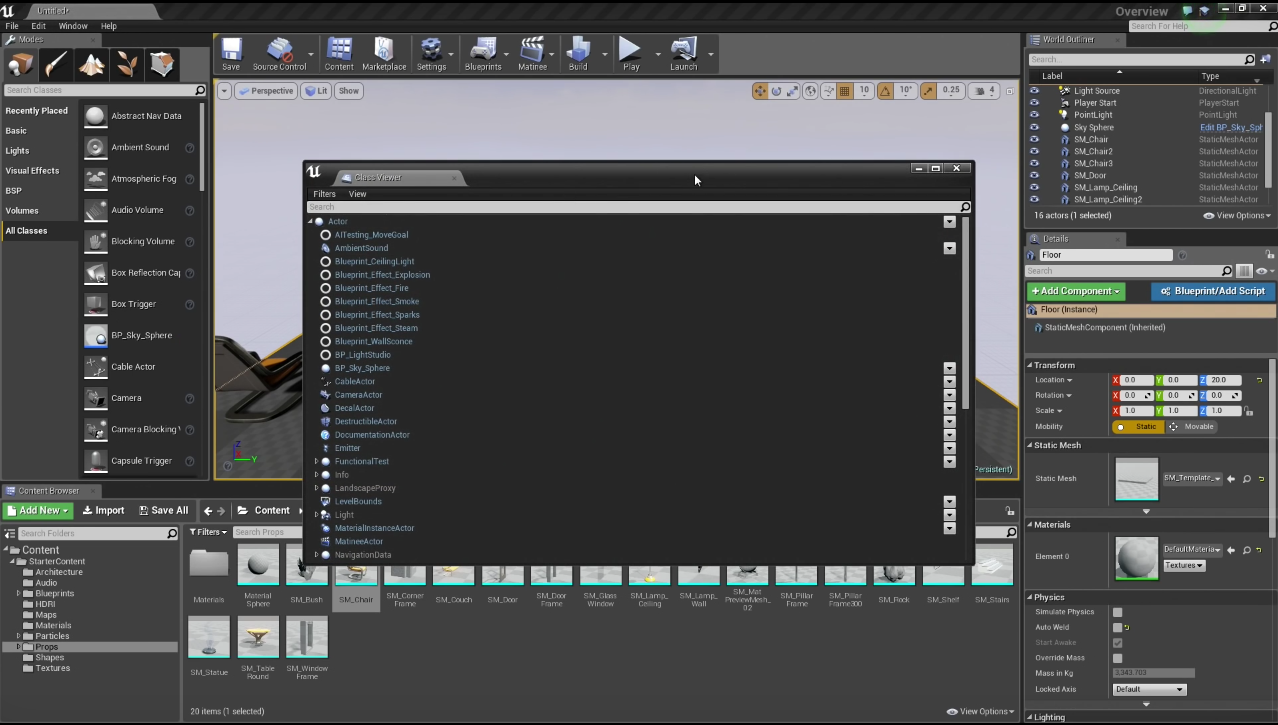
\includegraphics[height=12cm, width=16cm]{Capture4}
\caption{Class Viewer}
\end{figure}

\newpage

\subsection{Objekte bewegen}

\noindent In der Standardansicht werden bei jedem ausgew"ahltem Objekt die 3 Achsen angezeigt. Die rot/blau/gr"une Achse entspricht dabei jeweils der x/y/z-Achse. Per Klick auf eine der Achsen ist es m"oglich ein Objekt nur in die Richtung der gew"ahlten Achse zu verschieben (keine versehentliche Verschiebung in Richtung der beiden anderen Achsen). \newline
\noindent Zoomt man etwas genauer in das gew"ahlte Objekt hinein, sieht man jeweils eine Verbindung zwischen zwei Achsen, die es erm"oglicht, beide Achsen gleichzeitig auszuw"ahlen und in die Richtung beider Achsen zu schieben (ohne Verschiebung in Richtung der dritten Achse).\newline
\noindent Die wei"se Kugel im Urpsrung erm"oglicht eine Bewegung in Richtung aller drei Achsen. \newline
\newline
\noindent Hotkey-Tipp: Dr"ucken der End-Taste bei ausgew"ahltem Objekt setzt dieses direkt zur"uck auf den Boden. \newline
\newline
\noindent World Space: Die bisherigen Bewegungen haben alle im World Space stattgefunden, d.h. die Bewegung in x/y/z-Richtung erfolgt in x/y/z-Richtung  der Welt (immer gleich).  \newline
\noindent Local Space: Local Space bezeichnet die x/y/z-Richtung des K"orpers selbst. Im Normalfall sind diese identisch, ist ein Objekt aber jedoch rotiert, dann entsprechen die Richtungen nicht mehr einander. \newline
\newpage
\noindent In der rechten oberen Ecke des Viewports ist ein Globus-Symbol sichtbar, per Klick wechseln wir hier auf den Local-Space. Die Achsen werden nun entsprechend des gew"ahlten Objekts positioniert (siehe Bild). \newline
\newline
\newline
\begin{figure}
\
\includegraphics[height=8cm, width=16cm]{Capture6}
\caption{Achsen in Local Space}
\end{figure}
\newline
\noindent Shortcut-Tipp: Strg + ~ erm"oglicht schnelles Wechseln zwischen Local und World Space \newline
\newline
\noindent Wie bereits bekannt sein d"urfte, l"asst sich die Position nat"urlich auch rechts im Details Panel "andern. Hierbei ist zu beachten, dass standardm"a"sig eine Unreal-Einheit genau 1cm entspricht. Im Detail Panel l"asst sich im DropDown-Men"u auch die Bewegung zwischen 'World' und 'Relative' umschalten (Relative bezeichnet Position gegen"uber einem Parent-Objekt). \newline
\newpage
\noindent Grid Snapping: \newline
\newline
\noindent Grid Snapping eignet sich f"ur das genaue Anpassen zusammengeh"origer Objekte, wie zum Beispiel W"ande oder auch R"aume. Der Grid Snap Value ist ebenfalls in der rechten oberen Ecke des Viewports zu sehen und ist standardm"a"sig auf 10, d.h. wir bewegen ein Objekt immer um 10 Einheiten in die jeweilige Richtung. Der Wert kann nach Belieben angepasst werden, oder gar komplett ausgeschaltet werden.

\subsection{Objekte rotieren}

\noindent Wie im vorigen Kapitel gesehen, wird bei Auswahl eines Objekts zun"achst die drei Koordinatenachsen angezeigt. Ist das Objekt gew"ahlt, wechselt man durch dr"ucken der E-Taste in den Rotationsmodus. Statt den Achsen wird nun ein Rotationsgizmo angezeigt (Alternativ l"asst sich dies auch per Klick auf das Move Tool im Viewport "andern, die W-Taste wechselt zur"uck zu den Achsen).

\begin{figure}[h]
\includegraphics[height=7cm, width=16cm]{Capture7}
\caption{Rotationsb"ogen}
\end{figure}

\noindent Die drei farbigen B"ogen repr"asentieren Rotationsachsen. Analog zum Bewegen entlang einer Achse l"asst sich hier ein Bogen ausw"ahlen und anschlie"send das Objekt in diese Richtung rotiert werden. Nach Klicken und Halten eines Bogens wechselt die Sicht in den Kreiskompass. Hier l"asst sich beim Drehen genau ablesen, welchen Gradwert die aktuelle Rotation besitzt. Analgo zum Grid Snapping wird hier standardm"a"sig in 10° Schritten rotiert, auch dies kann man wahlweise anpassen. Rotationen sind ebenfalls abh"angig von Local und World Space und auch wie gewohnt im Detail Panel vertreten (Merkenf"ur Blueprints: Yaw = Z-Achse (blau), Pitch = Y-Achse (gr"un), Roll = X-Achse (rot)) 

\subsection{Objekte skalieren}

\noindent Um in den Skalierungsmodus zu wechseln, wird bei ausgew"ahltem Objekt die R-Taste gedr"uckt. Statt den urspr"unglichen Koordinatenachsen erhalten wir nun die Skalierungsachsen, die ebenfalls in x-y-z-Richtung zeigen (beim Skalieren immer in Local Space). Analog zum Bewegen eines Objektes k"onnen hier ein oder mehrere Achsen gew"ahlt werden und durch Ziehen mit der Maus in die jeweilige Richtung skaliert werden. \newline
\noindent Nat"urlich l"asst sich auch im Detail Panel skalieren. Hierbei ist die eingetragene Nummer entsprechend ein Vielfaches des Standardwertes '1' (Der Eintrag '3' bei z w"urde das Objekt in z-Richtung strecken, bis es die dreifache L"ange in dieser Richtung besitzt).\newline
\noindent Wie bei den beiden Tranformationen ist bei der Skalierung ebenfalls ein Snap-Value eingetragen, der nach Belieben angepasst oder ausgeschaltet werden kann. 
\subsection{Bewegen mit der Kamera}

\noindent Angenommen man m"ochte ein Objekt bewegen, der gew"unschte Zielort befindet sich aber au"serhalb des Sichtbereichs. Mit den bisherigen Kenntnissen w"urde man das Objekt bis an den Rand bewegen (per Drag$\&$Drop) , die Kamera bewegen und anschlie"send erneut das Objekt bewegen. Eine M"oglichkeit diesen Vorgang zu vereinfachen, ist das Objekt zu bewegen bei gedr"uckter SHIFT-Taste. In diesem Fall bewegt sich die Kamera mit dem Objekt mit. \newline
\noindent Eine weitere wichtige Funktion ist das 'Locking' der Kamera an bestimme Objekte, beispielsweise einer Lichtquelle. In der linken oberen Ecke befindet sich ein Pfeilsymbol, das ein Drop-Down-Men"u "offnet. Unter der Option 'Lock Viewport to Actor' l"asst sich das aktuell ausgew"ahlte Objekt anklicken. Die Kamera springt dann automatisch zu besagtem Objekt und man 'sieht' in Richtung des Objektes (beispielsweise in Richtung des Lichtstrahls, falls eine Lichtquelle gew"ahlt wurde).

\begin{figure}[h]
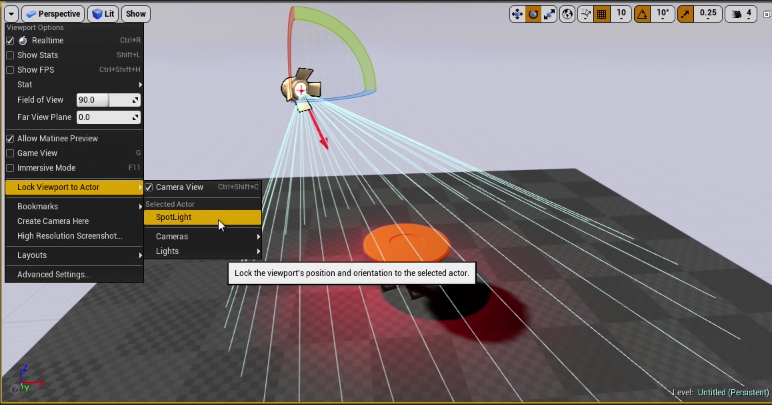
\includegraphics[height=6cm, width=16cm]{Capture8}
\caption{Vorteil beim Locking: Bewegen wir die Kamera, bewegt sich das gew"ahlte Objekt mit. Im selben Drop-Down-Men"u l"asst sich "uber 'Unlock' die Kamera wieder l"osen.}
\end{figure}

\subsection{Intro zum Content Browser}

\noindent Wie bereits erw"ahnt enth"alt der Content Browser alle Materials, Blueprints, Partikeleffekte und Meshes, sowie alle externen Assets. Sollte man versehentlich den Content Browser entfernt haben, l"asst es sich jederzeit in der Toolbar "uber dem Viewport "offnen (Alternativ Strg+Shift+F). Praktischweise ist der Content Browser links in mehrere Ordner unterteilt und mit einer Suchfunktion ausgestattet, die das Finden von Assets erleichtern. \newline
\newline
\noindent Externe Assets k"onnen jederzeit "uber den Import-Button importiert werden. Unreal unterst"utzt dabei eine Vielzahl von Formaten, die Liste ist unter 'Documentation' zu finden. Au"serdem k"onnen Assets auch direkt in den Ordner C/.../UE4$\_$Projects/'Projektname'/Content hinzugef"ugt werden. \newline

\subsubsection{Assets "uber den Content Browser editieren}

\noindent Eine der Hauptfeatures des Content Browsers ist die M"oglichkeit Assets zu editieren. Per Doppelklick auf ein Asset "offnet sich der entsprechende Editor, um das gew"ahlte Objekt zu bearbeiten. \newline
\newline
\noindent Static Meshes: \newline
\noindent Nach dem Doppelklick "offnet sich der Static Mesh Editor. Hier k"onnen Einstellungen f"ur Collisions vorgenommen, Materials hinzugef"ugt und Standardeinstellungen ver"andert werden. \newline
\newline
\noindent Blueprints: \newline
\noindent Der Blueprint Editor erm"oglicht es, die Abl"aufe der Blueprints zu modifizieren. Mehr zu Blueprints gibt es im entsprechenden Kapitel. \newline
\newline
\noindent Material Editor: \newline
\noindent Ebenfalls in Unreal enthaltener Sub-Editor, der die Bearbeitung von Materials erm"oglicht. 

\subsubsection{Navigation im Content Browser}

\noindent Dank den enthaltenen Sub-Editors ist es m"oglich, in Unreal neue Assets direkt selbst zu erstellen. "Uber den Buttron 'Add New' in der linken oberen Ecke l"asst sich jederzeit ein neues Objekt mit den bereits erw"ahnten Editors erstellen (Unter 'Add New' befinden sich auch einige n"utzliche Templates, unter anderem auch Blueprint Templates die direkt als Blueprints oder auch als C++ Version enthalten sind). Desweiteren ist es m"oglich jederzeit eigene Ordner in der links beigef"ugten Hierarchie anzulegen oder C++ Klassen einzuf"ugen, ebenfalls "uber den 'Add New' Button (Achtung: "Anderungen und Hinzuf"ugen mit dem 'Save all' Button speichern). \newline
\newpage
\noindent Im Ordnerverzeichnis an der linken Seite stehen uns auch einige Optionen (Rechtsklick auf leeren Bereich) zur Verf"ugung, allerdings sind diese gr"o"stenteils selbsterkl"arend. Wichtig ist allerdings die Option 'Connect to Source Control'. Hier kann man, falls ein gro"ses Team Source Control benutzt, sich jederzeit mit dieser verbinden bzw. die Verbindung trennen. \newline
\newline
\noindent Ein weiteres n"utzliches Feature ist die Lock-Funktion auf der rechten Seite des Content Browsers. Man nehme folgende Situation: Aus dem Ordner Static Meshes sollen K"orper hinzugef"ugt werden, anschlie"send dann verschiedene Materials eingef"ugt werden. Ist ein K"orper ausgew"ahlt, kann man per Klick auf das Lupen-Icon neben Material im Detail Panel ein Material hinzuf"ugen. Nach Klick auf die Lupe "offnet sich der entsprechende Ordner im Content Browser. M"ochte man nun laufend neue K"orper und Materials hinzuf"ugen, muss man zwischen diesen beiden Ordnern hin und her springen. Bet"atigt man aber vorher das Lock Icon im Content Browser, bleibt dieser auf den aktuell ausgew"ahlten Ordner. Dies erm"oglich es, viele Objekte aus verschiedenen Ordnern parallel einzuf"ugen, da nun nach dem Bet"atigen des Lupen-Icons ein neues Content Browser Fenster sich "offnet. Es k"onnen bis zu vier Content Browser gleichzeitig aktiv sein. \newline
\newline
\noindent Direkt links neben der 'Search Content'-Leiste befindet sich eine Filter-Option, die es ebenfalls einfacher macht, gesuchte Assets zu finden. Die Checkboxen k"onnen nach Belieben aktiviert/deaktiviert werden, die Ergebnisse werden unabh"angig von ihren jeweiligen Ordnern angezeigt.\newline
\noindent In der rechten unteren Ecke lassen sich au"serdem die 'View Options' bearbeiten, solle man die Anzeige des Content Browsers ver"andern wollen (Die 'Columns'-Ansicht enth"alt zu jedem Objekt weitere Informationen, die in der Tiles oder List-Ansicht nicht angezeigt werden). Hier lassen sich auch die Gr"o"se der Tiles skalieren und deren Thumbnails mit dem 'Thumbnail Edit Mode' ver"andern. Im aktivierten 'Thumbnail Edit Mode' l"asst sich auch die Form des Materials "andern, zum Beispiel von einer Sph"are zu einem W"urfel, per Klick auf die angezeigte Form direkt auf dem Thumbnail.

\begin{figure}[h]
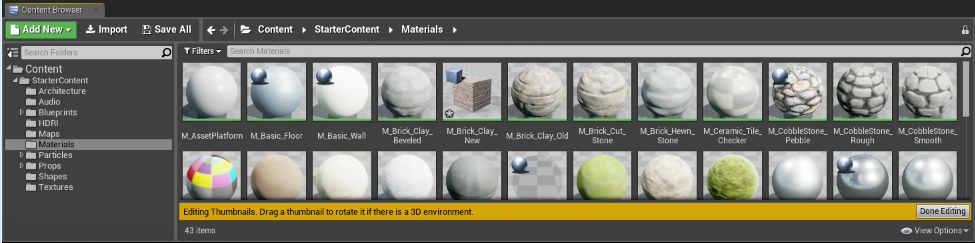
\includegraphics[height=5cm, width=15cm]{Capture9}
\caption{Content Browser im Thumbnail Edit Mode, in der linken oberen Ecke jedes Thumbnails l"asst sich die Form "andern}
\end{figure}

\section{Blueprints}

\noindent Blueprints sind die wichtigsten Hilfsmittel beim Entwickeln eines Spiels, gerade wenn Zeit eingespart werden soll oder auch die C++ Kenntnisse noch nicht ausreichend sind. Sie erm"oglichen die schnelle Implementierung h"aufig verwendeter Abl"aufe und sind gerade f"ur gescriptete Events optimal einzusetzen. Unreal Engine kommt mit vorgefertigten Blueprints, au"serdem ist es jederzeit m"oglich eigene Blueprints zu erstellen. Das Blueprint-System ist ausschlaggebend f"ur das Design eines Videospiels, sollte dennoch trotzdem als Kernfeature unserer Engine von allen beherrscht werden. Da ein Gro"steil unserer Animationen ebenfalls per Blueprint festgelegt werden, bitte ich alle darum, sich umfassend mit diesem Kapitel zu besch"aftigen.

\subsection{Einf"uhrung einfacher Blueprints}

\noindent Bevor man sich komplett in das Blueprint-System vertieft, sollte man zun"achst die bereits vorhandenen M"oglichkeiten innerhalb der Unreal Engine kennen. Unreal birgt bereits eine Vielzahl von Objekteigenschaften, die gerade f"ur Blueprints sp"ater notwendig.

\subsubsection{Destructible}

\noindent Die realistische Zerst"orung von Objekten ist meist ein schwieriges Unterfangen. F"ur Static Meshes hat Unreal bereits ein physikgetreues Modell, dass die einfache Erzeugung von Destructibles erm"oglicht. Im Content Browser per Rechtsklick das jeweilige Mesh ausw"ahlen und im Pop-Up-Men"u die Option 'Create Destructible-Mesh' ausw"ahlen. 

\begin{figure}[h]
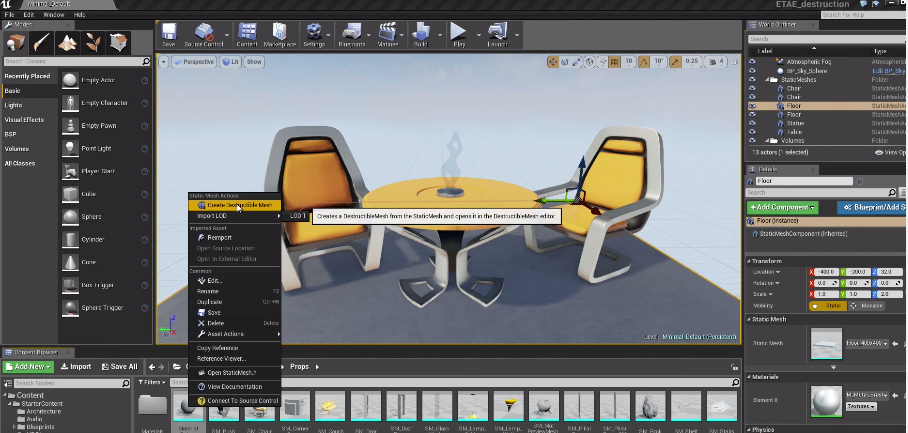
\includegraphics[height=7cm, width=15cm]{Capture10}
\caption{Erzeugung eines Destructibles}
\end{figure}


\noindent Das gew"ahlte Mesh wird dupliziert und mit einer kleinen rosa Leiste im Content Browser angezeigt. Alle Objekte mit dieser rosa Leiste sind Destructibles, per Doppelklick l"asst sich der Destructible Editor "offnen. \newline
\noindent Hier lassen sich auf der rechten Seite Einstellungen f"ur das Destructible vornehmen. Uns interessiert hier zun"achst mal das Feld 'Cell Site Count'. Hier l"asst sich die Anzahl der Zellen festlegen, und somit die Feinheit des Zerfalls (Achtung: Gr"o"sere Zahl hier bedeutet mehr Berechnungen $\rightarrow$ Perfomanz). "Uber den Button 'Fracture Mesh' in der oberen linken Ecke wird anschlie"send das Mesh als zerst"ortes Mesh angezeigt. "Uber den Schieberegler 'Explode Amount' kann man den Zerfall beobachten. \newline
\newline
\noindent Ein paar weitere Einstellungen sind hier wichtig: \newline
\noindent - Damage Threshold: Hier l"asst sich festlegen, bei welchem Schaden, dass Objekt zerf"allt \newline
\noindent - Enable Impact Damage: Wenn aktiviert, nimmt das Objekt bei physikalischer Aktion  Schaden. \newline
 \noindent- Impact Damage: Physikalischer Schaden das Objekt wahrnehmen kann, bevor es zerbricht. \newline

\subsubsection{Camerashake}

\noindent Ein Camera-Shake-Effekt erm"oglicht es auf einfache Weise gro"se Vibrationen darzustellen, um so zum Beispiel einer Explosion Nachdruck zu verleihen.Damit wir diesen Effekt einmal selber implementieren, laden wir das First-Person-Template als Projekt. \newline
\newline
\noindent Wir beginnen damit, dass wir per Rechtsklick in den Content Browser die Funktion 'Blueprint Class' ausw"ahlen, um ein neues Blueprint zu erstellen. "Uber Suche l"asst sich die Camera-Shake-Klasse schnell finden, ausw"ahlen und dann "offnen. Nun kann man das Template nach belieben benennen und anschlie"send im Blueprint Editor "offnen. Wir beachten wieder die Attribute auf der rechten Seite. \newline
\newline
\noindent Oscillation Duration: Dauer des Camera-Shakes \newline
\noindent Rotation Oscillation: Gibt dem Shake auch eine gewisse Rotation (Pitch, Yaw,Roll) \newline
\noindent Location Oscillation: Die Oszillation in x/y/z-Richtung \newline
\newline
\noindent Nach Eingabe der Werte erst kompilieren ('Compile') und anschlie"send speichern. \newpage
\noindent Wir "offnen nun den Blueprint FirstPersonCharakter im Blueprint-Editor. Das untere Rechteck beinhaltet alle Blueprints, die beim abfeuern der Waffe ben"otigt werden. Ganz am Ende der Blueprint-Kette 'Play Sound at Location' wollen wir nun den Camera-Shake hinzuf"ugen. Mit der Maus k"onnen wir an dem nicht-gef"ulltem Pfeilsymbol eine neue Linie ziehen und somit ein neues Node platzieren. Nachdem man die Linie mit der Maus gezogen hat, "offnet sich ein Suchfenster. Durch Eingabe von 'shake' finden wir das Node 'Play World Camera Shake' und w"ahlen dieses aus. Es wird damit direkt ein neues Node platziert.

\begin{figure}[h]
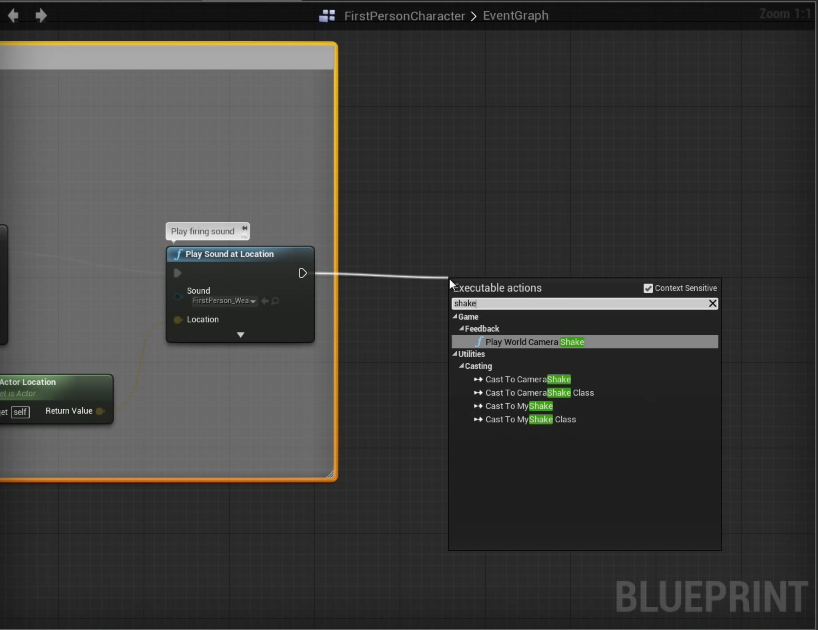
\includegraphics[height=8cm, width=15cm]{Capture11}
\caption{Neuen Node platzieren}
\end{figure}

\noindent Der platzierte Node besitzt eine Menge von Eigenschaften, darunter 'Shake'. Hier definieren wir die benutzte Klasse f"ur den Shake-Effekt. Die von uns neu erstellte Shake-Klasse kann dann hier ausgew"ahlt werden. Nun brauchen wir noch eine Location, an der besagter Shake ablaufen wird (Epicenter). Im bereits implementierten FirstPersonCharacter-Blueprint befindet sich das Node 'Get Actor Location'. Wir verbinden diesen Node mit unserem Node, damit der Shake die jeweilige Position erh"alt. Die anderen Werte sind erstmal zweitrangig. \newline
\noindent Wenn wir das ganze nun abspeichern und zur"uck zu unserem Spiel wechseln, wird jetzt bei jedem Schuss eine Vibration der Kamera stattfinden.
\newpage

\subsubsection{Timer}

\noindent Timer k"onnen in vielen Situationen hilfreich sein. Sie erm"oglichen das Ablaufen bestimmter Ereginisse in einem definierten Zeitintervall ein- oder mehrmals. Um den Timer zu implementieren, benutzen wir hier eine Lichtquelle, dessen Farbe wir in bestimmten Zeitabst"anden ver"andern. \newline \newline
\noindent Ist ein Objekt ausgew"ahlt, wird wie gewohnt rechts das Detail Panel angezeigt. F"ur jedes Objekt haben wir hier die M"oglichkeit einen Komponenten hinzuzuf"ugen ('Add Component') oder eine Blueprint-Klasse zu erzeugen, die dieses Objekt enth"alt ('Blueprint/Add Script'). Wir w"ahlen also unsere Lichtquelle und erstellen eine Blueprint-Klasse "uber den blauen Blueprint-Button im Detail-Panel. \newline \newline
\noindent Die erstellte Blueprint-Klasse ist nun im Content Browser zu finden. Zum Bearbeiten "offnen wir die Klasse im Blueprint-Editor. Im Viewport wird uns die gew"ahlte Lampe angezeigt, zum Bearbeiten der Abl"aufe ben"otigen wir den Event Graph, welcher einer der Tabs "uber dem Viewport ist. Hier sehen wir die vetraute Form des Blueprint-Editors mit den Nodes, noch ohne Verbindungen. \newline
\newline
\noindent Um den Ablauf bei Beginn zu starten, ziehen wir erstmal eine Linie vom Node 'Event Begin Play'. Im folgenden Men"u suchen wir nach dem Blueprint 'SetLightColor(PointLightComponent)' bzw. SetLightColor(benutzte Lichtquelle). Im neuen Node ist nun eine neue Farbe nach dem Wechsel einzugeben. Wir m"ochten diese Farbe zuf"allig w"ahlen, dazu "offnen wir per Rechtsklick erneut das Nodemen"u und w"ahlen den Node 'Random Vector' (Farbe ist ein Vektor RBG). Um den zuf"alligen Vektor nun noch in einen g"ultigen Farbvektor zu formen, erstellen wir das Node 'ToLinearColor'. Jetzt k"onnen wir Node 'Random Vector' mit Node 'ToLinearColor' verbinden und dieses anschlie"send an das Attribut 'New Light Color' unseres Blueprints 'SetLightColor' ankn"upfen. \newline
\newline
\noindent Hinweis: Der Timer ist zwar noch nicht implementiert, aber wenn wir jetzt zur"uck im Editor auf 'Play' klicken, hat unsere Lichtquelle einen zuf"alligen Farbwert. \newline
\newline
\noindent Um den Timer zu implementieren, ziehen wir erneut eine Linie vom Node 'Event Begin Play' und f"ugen das Blueprint 'SetTimer' an. Die Attribute sollten selbsterkl"arend sein, es ist darauf zu achten, dass Looping aktiviert ist, damit die Farbe sich wiederholend "andert. 'Function Name' bezeichnet welche Funktion aufgerufen wird. Wir erstellen per Rechtsklick ein 'Custom Event' und benennen es beispielsweise RandomCol. Wir verbinden RandomCol mit unserer vorher erstellten SetLightColor und k"onnen dann beim Timer den FunctionName 'RandomCol' benutzen(Kompilieren und Speichern nicht vergessen).

\newpage
\begin{figure}[h]
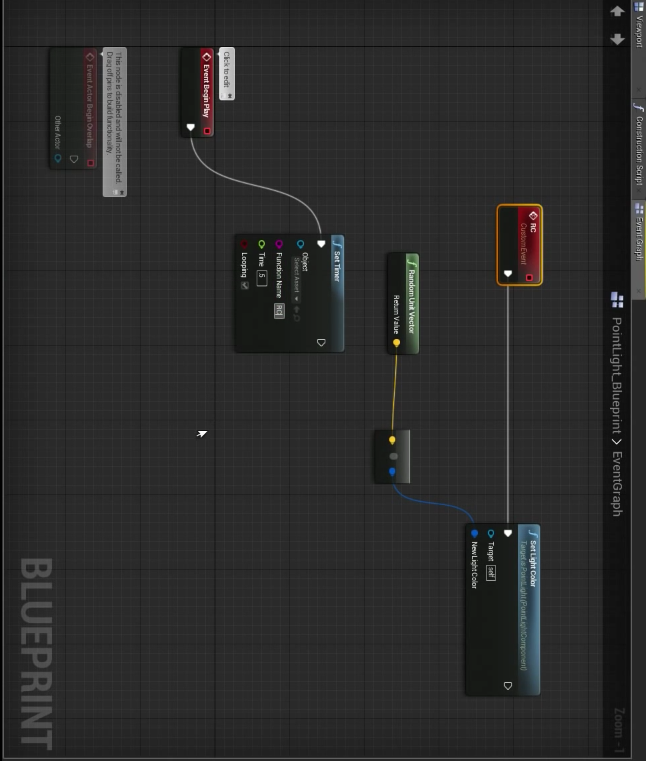
\includegraphics[height=14cm, width=15cm]{Capture12}
\caption{Nodes f"ur Lichtwechsel in bestimmtem Zeitabstand}
\end{figure}
\subsubsection{Slow Motion Effect}

\noindent Wir starten erneut mit einem neuen Projekt und laden das First Person Template. Um den Slow-Motion Effekt einzuf"ugen, "offnen wir FirstPersonCharacter im Blueprint-Editor und erstellen ein neues Node 'Event Tick' (wie gewohnt per Rechtsklick und anschlie"send "uber die Suchleiste). Event Tick ist ein Node, dass f"ur jeden Frame aufgerufen wird. \newline
\newline
\newline
\noindent Wir erstellen ein zweites Node 'Execute Console Command', welche wir ben"otigen werden, um den Slow-Motion-Effekt an unseren Charakter anzupassen . Au"serdem ben"otigen wir ein drittes Node 'Build String(float)', welches "uber Return Value an das Command-Attribut des Execute Console Command verkn"upft ist (das Prefix slomo ist ein Shortcut zum Console Command f"ur die Zeitlupe).

\begin{figure}[h]
\includegraphics[height=8cm, width=15cm]{Capture13}
\caption{Prefix 'slomo' , float-Wert soll vom Charakter abh"angig sein}
\end{figure}

\noindent Um den float-Wert an den Charakter anzupassen, erstellen wir ein neues Node 'Get Velocity'. Der return-value von Velocity ist ein Vektor, den wir nicht als float benutzen k"onnen, allerdings k"onnen wir wiederrum das Node 'Vector length' aufrufen, der die L"ange des Vektors berechnet. Diesen k"onnen wir allerdings noch nicht an den float-Wert kn"upfen, da sich die L"ange des Vektors nicht zwischen 0 und 1 befindet. Links im Reiter Components finden wir die Komponente CharacterMovement, hier k"onnen wir einsehen, dass die minimale Geschwindigkeit unseres Charakters 0 und die maximale Geschwindigkeit 600 ist. Diese Werte ben"otigen wir f"ur den Node 'Map Range', welchen wir jetzt erstellen. Als In Range geben wir 0 f"ur A und 600 f"ur B ein, als Out Range 0 und 1. Dies bedeutet, dass unsere Vector Length auf Werte zwischen 0 und 1 gemappt wird, solange die Input-Werte zwischen 0 und 600 liegen.

\newpage

\begin{figure}[h]
\includegraphics[height=8cm, width=15cm]{Capture14}
\caption{Slow-Motion abh"angig von Geschwindigkeit des Charakters}
\end{figure}

\noindent In diesem Beispiel ist das Spiel sehr langsam, wenn der Spieler sich kaum/nicht bewegt, aber kaum auffallend wenn der Spieler sich schnell bewegt. Analog zu vorigen Beispielen kann der Slow-Motion-Effekt unabh"angig von der Spielergeschwindigkeit sein und entweder als Funktion aufgerufen werden (siehe CameraShake) oder auch an einen Timer gekoppelt werden.

\subsubsection{Jump Pad}

\noindent Zu Beginn w"ahlen wir das Third-Person-Template und erzeugen wie bereits bekannt "uber den Content Browser eine neue Blueprint-Class vom Typ 'Actor'. Anschlie"send wird die neue Klasse benannt und im Blueprint-Editor ge"offnet. \newline
\newline
\noindent Zu Beginn braucht unser Jump Pad ein Mesh, welches das Pad repr"asentieren soll. "Uber 'Add Component' f"ugen wir der Einfachheit halber das Basic Component  Cylinder. Per Scaling im Panel rechts passen wir die Dimensionen entsprechend unserer Vorstellung an (Traditionelle Jump Pads sind Zylinder mit sehr kleiner H"ohe). Ebenfalls im rechten Panel unter dem Reiter l"asst sich die Einstellung 'Collision Presets'. Standardm"a"sig ist diese Option auf 'BlockAllDynamic' , was nat"urlich  f"ur ein Jump Pad eher kontraproduktiv ist. Beim Jump Pad wollen wir die M"oglichkeit haben, es mit dem Spieler zu "uberlappen aber trotzdem das Event zu erzeugen. Die gew"unschte Einstellung ist also 'OverlapAllDynamic', aber die Option  'Generate Overlap Events' sollte aktiviert bleiben(Kompilieren und Speichern nicht vergessen).  \newline
\newline
\noindent Den neuen Actor k"onnen wir jetzt in unsere Szene positionieren. Noch wird nichts passieren, da wir ja kein Event f"ur den Overlap definiert haben. Dazu wechseln wir wieder in den Blueprint-Editor und w"ahlen den Event-Graphen. Wir erstellen das Node 'Event Actor Begin Overlap'. Dieser Node wird jedes mal aufgerufen, wenn ein anderer Actor sich mit dem jetzigen "uberlappt. "Uber das Attribut 'Other Actor' k"onnen wir festlegen, welche anderen Actors das Event ausl"osen k"onnen. In diesem Beispiel setzen wir an dieses Attribut nur unseren ThirdPersonCharacter (neues NodeCast to ThirdPersonCharacter, verbinden). Nat"urlich k"onnen auch andere Objekte als Eventausl"oser festgelegt werden, zum Beispiel Kisten oder "ahnliches. An den Charakter k"onnen wir das Blueprint 'Launch Character' andocken. In dem Node 'Launch Character' k"onnen wir die Geschwindigkeit des Sprungs in x,y,z-Richtung definieren (Ein Sprung entspricht nur einem z-Wert $\rightarrow$ vertikal). Einen beliebigen Wert eingeben, kompilieren und speichern. Beim Starten wird unser Charakter nun jedes mal, wenn er das Jump Pad ber"uhrt, in die Luft geschleudert.

\begin{figure}[h]
\includegraphics[height=4cm, width=15cm]{Capture15}
\caption{Blueprint f"ur das Jump Pad}
\end{figure}

\subsubsection{Hover-Komponente}

\noindent 


\subsubsection{Simples Conveyor Volumen}
\subsubsection{Komponenten f"ur Game-Behaviour}





\end{document}